\documentclass{beamer}

\usepackage[T1]{fontenc}
\usepackage[utf8]{inputenc}
\usepackage[american]{babel}
\usepackage{amsmath,amssymb,amsthm}
\usepackage{tikz,pgflibraryarrows,pgflibraryplotmarks,pgflibrarysnakes,pgflibraryshapes}
\usepackage[backend=biber,citestyle=authoryear-comp,bibstyle=beamer,doi=false,isbn=false,url=false,maxnames=10]{biblatex}
\usepackage[nosfdefault]{comicneue}
\bibliography{defeo}

\mode<presentation>{%
  \usetheme{Boadilla}
}
\beamertemplatenavigationsymbolsempty

\usepackage{sourcesanspro}
\usepackage[amssymb,amsfonts]{concmath}
\usefonttheme[onlymath]{serif}

\renewcommand{\emph}[1]{{\usebeamercolor[fg]{structure}#1}}

%\let\footcite\footnote

\newcommand{\C}{\mathbb{C}}
\newcommand{\R}{\mathbb{R}}
\newcommand{\Z}{\mathbb{Z}}
\newcommand{\N}{\mathbb{N}}
\newcommand{\Q}{\mathbb{Q}}
\newcommand{\F}{\mathbb{F}}
\renewcommand{\O}{\mathcal{O}}
\newcommand{\tildO}{\mathcal{\tilde{O}}}
\newcommand{\End}{\operatorname{End}}
\newcommand{\chr}{\operatorname{char}}
\newcommand{\Cl}{\operatorname{Cl}}
\renewcommand{\a}{{\mathfrak{a}}}
\renewcommand{\b}{{\mathfrak{b}}}
\newcommand{\cyc}[1]{{\langle #1 \rangle}}
\newcommand{\ord}{\operatorname{ord}}

\usetikzlibrary{matrix,decorations,decorations.text,calc,arrows,snakes,shapes,positioning}

\pgfkeys{/triangle/.code=\tikzset{x={(-0.5cm,-0.866cm)},y={(1cm,0cm)}}}
\pgfkeys{/lattice/.code n args={4}{\tikzset{cm={#1,#2,#3,#4,(0,0)}}}}

\newcommand{\axes}[4]{
  \clip (#1,#3) rectangle (#2,#4);
  \draw [thin, gray, -latex] (#1,0) -- (#2,0);% Draw x axis
  \draw [thin, gray, -latex] (0,#3) -- (0,#4);% Draw y axis
}

\newcommand{\lattice}[2]{
  \draw[style=help lines,dashed] (#1-1,#1-1) grid[step=1] (#2+1,#2+1);
  \foreach \x in {#1,...,#2}{
    \foreach \y in {#1,...,#2}{
      \node[draw,circle,inner sep=2pt,fill] at (\x,\y) {};
      % Places a dot at those points
    }
  }
}

\newcommand{\bl}[1]{\textcolor{blue}{#1}}
\newcommand{\rd}[1]{\textcolor{red}{#1}}
\newcommand{\gr}[1]{\textcolor{green}{#1}}

% This command defines a triangle of dots of given height
\newcommand{\dottriangle}[2][\i-\j]{%
  \foreach \i in {0,...,#2} {%
    \foreach \j in {0,...,\i} {%
      \draw(\i,\j) node{#1};%
    }%
  }}


\title{Isogeny based cryptography}
\author{Luca De Feo}
\date[UVSQ, Sep 19, 2018]{Sep 19, 2018, Évaluation HCERES, UVSQ}
\institute[UVSQ]{Université Paris Saclay -- UVSQ}

\begin{document}

\frame[plain]{\titlepage}

%% 

\begin{frame}{Diffie--Hellman key exchange}
  \begin{description}
  \item[Goal:] Alice and Bob have never met before. They are chatting
    over a public channel, and want to agree on a \emph{shared secret}
    to start a private conversation.
  \item[Setup:] They agree on a (large) cyclic group
    $G=\langle g\rangle$ of order $N$.
  \end{description}

  \begin{center}
    \begin{tikzpicture}
      \node at (0,0) {\bf Alice};
      \node at (7,0) {\bf Bob};
      \node at (0,-1) {pick random \alert{$a\in\Z/N\Z$}};
      \node at (0,-1.5) {compute $A=g^a$};
      \node at (7,-1) {pick random \alert{$b\in\Z/N\Z$}};
      \node at (7,-1.5) {compute $B=g^b$};
      \draw[->]
      (1,-2) to node[auto] {$A$} (6,-2);
      \draw[->] (6,-2.5) to node[auto] {$B$} (1,-2.5);
      \node at (3.5,-3.5) {\emph{Shared secret} is \alert{$B^a=g^{ab}=A^b$}};
    \end{tikzpicture}
  \end{center}
\end{frame}

%%

\begin{frame}{Brief history of DH key exchange}
  \begin{description}
  \item[1976] Diffie \& Hellman publish \emph{New directions in
      cryptography}, suggest using $G=\F_p^\ast$.
  \item[1978] Pollard publishes his \emph{discrete logarithm}
    algorithm ($O(\sqrt{\# G})$ complexity).
  \item[1980] Miller and Koblitz independently suggest using
    \emph{elliptic curves} $G=E(\F_p)$.
  \item[1994] Shor publishes his \emph{quantum discrete logarithm /
      factoring} algorithm.
  \item[2005] NSA standardizes elliptic curve key agreement (ECDH) and
    signatures ECDSA.
  \item[2017] $\sim 70\%$ of web traffic is secured by ECDH and/or
    ECDSA.
  \item[2017] NIST launches \emph{post-quantum competition}, says
    ``not to bother moving to elliptic curves, if you haven't yet''.
  \end{description}
\end{frame}

%%

\begin{frame}{History of isogeny-based cryptography}
  \begin{description}
  \item[1996] Couveignes introduces the \emph{Hard Homogeneous
      Spaces}. His work stays unpublished for 10 years.
  \item[2006] Rostovtsev \& Stolbunov independently rediscover
    Couveignes ideas, suggest isogeny-based Diffie--Hellman as a
    \emph{quantum-resistant} primitive.
  \item[2006-2010] Other isogeny-based protocols by Teske and Charles,
    Goren \& Lauter.
  \item[2011-2012] D., Jao \& Plût introduce \emph{SIDH}, an
    efficient post-quantum key exchange inspired by Couveignes,
    Rostovtsev, Stolbunov, Charles, Goren, Lauter.
  \item[2017] SIDH is submitted to the NIST competition (with the name
    \emph{SIKE}, only isogeny-based candidate).
  \item[2018] D., Kieffer \& Smith \textit{resurrect} the
    Couveignes--Rostovtsev--Stolbunov protocol, Castryck, Lange,
    Martindale, Panny \& Renes publish an efficient variant named
    \emph{CSIDH}.
  \end{description}
\end{frame}

%%

\begin{frame}{Elliptic curves}

  Let \emph{$E \;:\; y^2 = x^3 + ax + b$} be an elliptic curve\dots

  \begin{center}
    \begin{tikzpicture}[domain=-2.4566:4,samples=100]
      \newcount\rotate
      \animate<2-6>
      \animatevalue<2-6>{\rotate}{0}{90}
      \begin{scope}[rotate=-\the\rotate]
        \draw plot (\x,{0.5*sqrt(\x*\x*\x-4*\x+5)});
        \draw plot (\x,{-0.5*sqrt(\x*\x*\x-4*\x+5)});
      \end{scope}
      
      \begin{uncoverenv}<1>
        \begin{scope}[yscale=1/2]
          \draw[thin,gray,-latex] (0,-7) -- (0,7);
          \draw[thin,gray,-latex] (-3,0) -- (4,0);
          
          \draw (-3,1) -- (4,8/3+3);
          \begin{scope}[every node/.style={draw,circle,inner sep=1pt,fill},cm={1,2/3,0,0,(0,3)}]
            \node at (-2.287980,0) {};
            \node at (-0.535051,0) {};
            \node at (3.267475,0) {};
          \end{scope}
          \begin{scope}[every node/.style={yshift=0.3cm},cm={1,2/3,0,0,(0,3)}]
            \node at (-2.287980,0) {$P$};
            \node at (-0.535051,0) {$Q$};
            \node at (3.267475,0) {$R$};
          \end{scope}
          \draw[dashed] (3.267475,3.267475*2/3+3) -- (3.267475,-3.267475*2/3-3) 
          node[draw,circle,inner sep=1pt,fill] {}
          node[xshift=-0.1cm,anchor=east] {$P+Q$};
        \end{scope}
      \end{uncoverenv}
    \end{tikzpicture}
  \end{center}
\end{frame}

%%

\begin{frame}{Elliptic curves}
  \transdissolve
  \centering
  
\includegraphics[height=0.7\textheight]{ec-happy}
\end{frame}

%%

\begin{frame}{The QUANTHOM Menace}
  \centering
  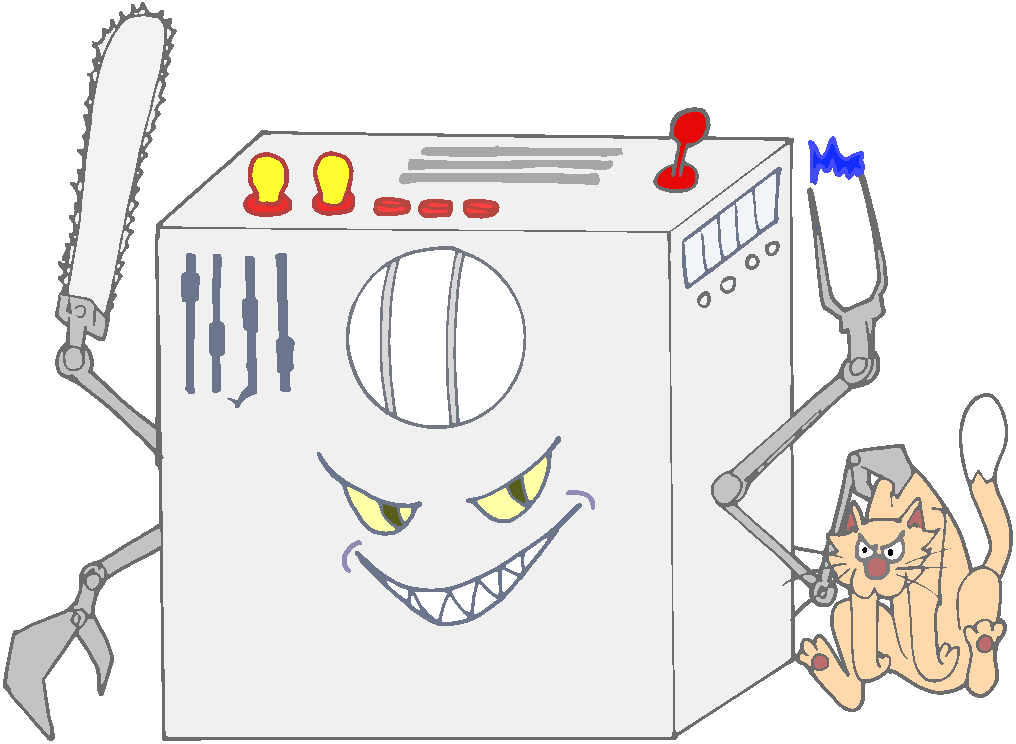
\includegraphics[height=0.7\textheight]{qc-color}
\end{frame}

%%

\begin{frame}{Basically every isogeny-based protocol...}
  \centering
  \begin{tikzpicture}
    \comicneue\itshape
    \node at (0,0) {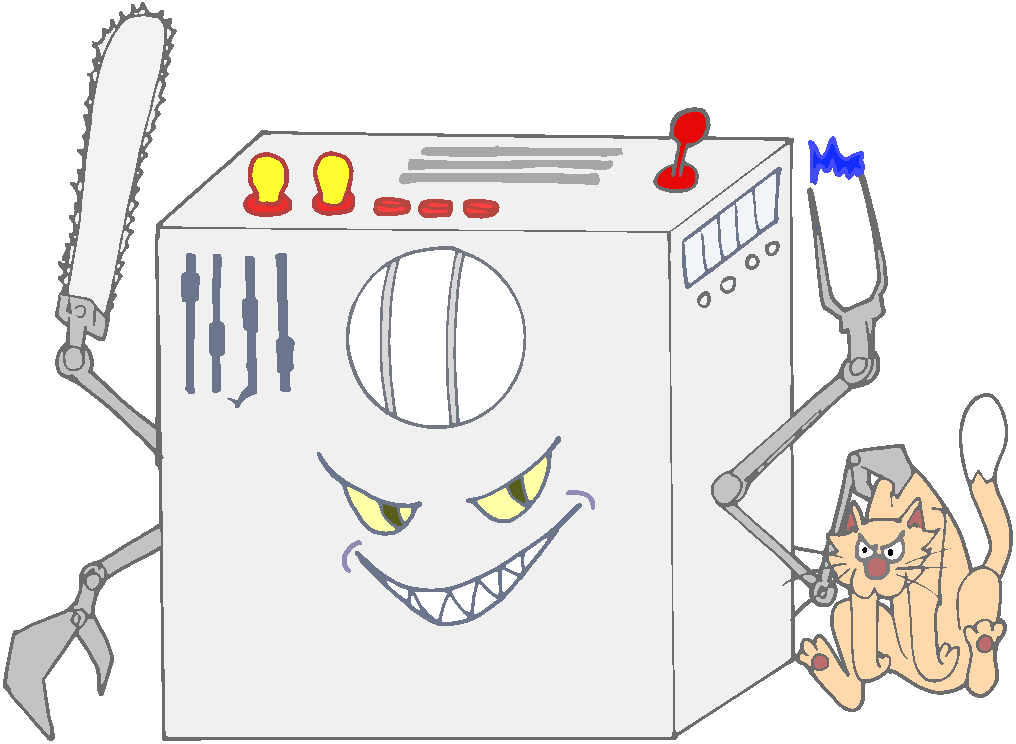
\includegraphics[height=2.5cm]{qc-color}};
    
    \node(E0) at (-5,0) {
\includegraphics[height=1cm]{ec-happy}};

    \uncover<2->{
      \node(EA) at (0,3.5) {
\includegraphics[height=1cm]{ec-happy}};
      \node(EB) at (0,-3.5) {
\includegraphics[height=1cm]{ec-happy}};
      \draw[->,decorate,decoration=snake] (E0) to (EA);
      \draw[->,decorate,decoration=snake] (E0) to (EB);
      \node[right=0.3cm of EA] {\bl{Public curve}};
      \node[right=0.3cm of EB] {\bl{Public curve}};
    }
    \uncover<3>{
      \node(ES) at (5,0) {
\includegraphics[height=1cm]{ec-happy}};
      \draw[->,decorate,decoration=snake] (EA) to (ES);
      \draw[->,decorate,decoration=snake] (EB) to (ES);
      \node[below=1em of ES] {\rd{Shared secret}};
    }
  \end{tikzpicture}
\end{frame}

%%

\begin{frame}
  \frametitle{What's an isogeny?}

  Isogenies are just \alert{the right notion\texttrademark{} of
    morphism} for elliptic curves

  \begin{itemize}
  \item Surjective group morphisms.
  \item Algebraic maps (i.e., defined by polynomials).
  \end{itemize}

  (Separable) isogenies $\Leftrightarrow$ finite subgroups:
  \alert{\[0 \to H \to E \overset{\phi}{\to} E' \to 0\]}
  The kernel \emph{$H$} determines the image curve \emph{$E'$} up to
  isomorphism \[\emph{E/H\overset{\text{\tiny def}}{=}E'}.\]
\end{frame}

%% 

\begin{frame}{Isogenies: an example over $\F_{11}$}
  \begin{tikzpicture}[scale=0.4]
    \begin{scope}
      \node[anchor=center] at (0,7) {$E \;:\; y^2 = x^3 + x$};

      \uncover<-1>{
        \draw[thin,gray] (0,-6) -- (0,6);
        \draw[thin,gray] (-6,0) -- (6,0);
      }

      \foreach \x/\y in {0/0,5/3,-4/3,-3/5,-2/1,-1/3} {
        \draw[blue,fill] (\x,\y) circle (0.2) node(E_\x_\y){}
        (\x,-\y) circle (0.2) node(E_\x_-\y){};
      }

      \uncover<2->{\draw[red,fill] (0,0) circle (0.3);}
    \end{scope}

    \draw[black!10!white,thick] (8,-7) -- +(0,14);
    
    \begin{scope}[shift={(16,0)}]
      \node at (0,7) {$E' \;:\; y^2 = x^3 - 4x$};

      \uncover<-1>{
        \draw[thin,gray] (0,-6) -- (0,6);
        \draw[thin,gray] (-6,0) -- (6,0);
      }

      \foreach \x/\y in {0/0,2/0,3/2,4/2,6/4,-2/0,-1/5} {
        \draw[color=blue,fill] (\x,\y) circle (0.2) node(F_\x_\y){}
        (\x,-\y) circle (0.2) node(F_\x_-\y){};
      }
    \end{scope}

    \begin{scope}[color=red,-latex,dashed]
      \begin{uncoverenv}<2->
        \path
        (E_5_3) edge (F_3_2)
        (E_-4_3) edge (F_4_-2)
        (E_-3_5) edge (F_4_2)
        (E_-2_1) edge (F_3_-2)
        (E_-1_3) edge (F_-2_0);
      \end{uncoverenv}
      \begin{uncoverenv}<2->
        \path
        (E_5_-3) edge (F_3_-2)
        (E_-4_-3) edge (F_4_2)
        (E_-3_-5) edge (F_4_-2)
        (E_-2_-1) edge (F_3_2)
        (E_-1_-3) edge (F_-2_0);
      \end{uncoverenv}
    \end{scope}
  \end{tikzpicture}
  
  \begin{columns}
    \begin{column}{0.5\textwidth}
      \[\phi(x,y) = \left(\frac{x^2 + 1}{x},\quad y\frac{x^2-1}{x^2}\right)\]
    \end{column}
    \begin{column}{0.5\textwidth}
      \begin{itemize}
      \item<2-> Kernel generator in \alert{red}.
      \item<2-> This is a degree $2$ map.
      \item<2-> Analogous to $x\mapsto x^2$ in $\F_q^*$.
      \end{itemize}
    \end{column}
  \end{columns}
\end{frame}

%%

\begin{frame}
  \frametitle{Isogeny graphs}
  
  \vspace{-2mm}

  \begin{columns}
    \begin{column}{0.65\textwidth}
      We look at the graph of elliptic curves with isogenies \emph{up
        to isomorphism}.  We say two \alert{isogenies} $\phi,\phi'$
      are \alert{isomorphic} if:
    \end{column}
    \begin{column}{0.3\textwidth}
      \begin{center}
        \begin{tikzpicture}[node distance=4em]
          \node(E){$E$}; 
          \node(E1)[right of=E]{$E'$};
          \node(E2)[below of=E1]{$E'$};
          \scriptsize
          \path[->] (E) edge node[auto]{$\phi$} (E1);
          \path[->] (E) edge node[auto,swap]{$\phi'$} (E2);
          \path[<->] (E1) edge node[rotate=270] {\large$\widetilde{}$} (E2);
        \end{tikzpicture}
      \end{center}
    \end{column}
  \end{columns}

  \emph{Example:} Finite field, ordinary case, graph of isogenies of degree $3$.

  \begin{center}
    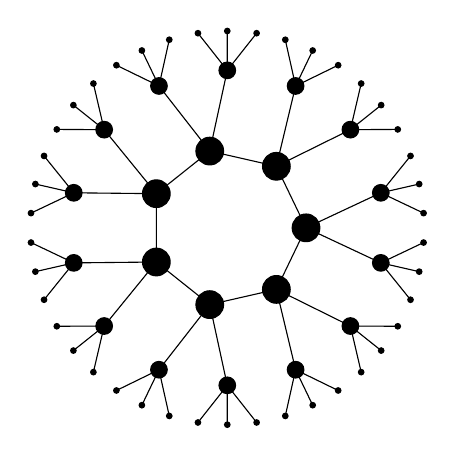
\begin{tikzpicture}[]
      \begin{scope}
        \def\crater{7}
        \foreach \i in {1,...,\crater} {
          \draw[fill] (360/\crater*\i:1cm) circle (5pt);
          \draw (360/\crater*\i : 1cm) -- (360/\crater*\i+360/\crater : 1cm);
          \foreach \j in {-1,1} {
            \draw[fill] (360/\crater*\i : 1cm) -- (360/\crater*\i + \j*360/\crater/4 : 2cm) circle (3pt);
            \foreach \k in {-1,0,1} {
              \draw[fill] (360/\crater*\i + \j*360/\crater/4 : 2cm) --
              (360/\crater*\i + + \j*360/\crater/4 + \k*360/\crater/6 : 2.5cm) circle (1pt);
            }
          }
        }
      \end{scope}
    \end{tikzpicture}
  \end{center}
\end{frame}

%%

\begin{frame}
  \frametitle{Structure of the graph}
  
  \begin{theorem}[Serre-Tate]
    Two curves are isogenous over a finite field $k$ if and only if
    they have the \alert{same number of points} on $k$.
  \end{theorem}
  \vspace{-0.6em}
  \begin{block}{The graph of isogenies of \alert{prime} degree \alert{$\ell\ne p$}}
    \small
    \vspace{-1em}
    \begin{tabular}{p{0.17\textwidth} p{0.8\textwidth}}
      \raggedright
      \emph{Ordinary case (isogeny volcanoes)}
      & \vspace{-1em}
        \begin{itemize}
          \setlength\itemsep{-0.6ex}
        \item Nodes can have degree \emph{$0,1,2$} or \emph{$\ell+1$}.
          \begin{itemize}
          \item  For $\sim 50\%$ of the primes $\ell$, graphs are just isolated
            points;
          \item For other $\sim 50\%$, graphs are $2$-regular;
          \item other cases only happen for finitely many $\ell$'s.
          \end{itemize}
        \end{itemize}
      \\[-1.4em]
      \raggedright
      \emph{Supersingular case ($\F_p$)}
      & \vspace{-1.2em}
        \begin{itemize}
          \setlength\itemsep{-0.6ex}
        \item If $\ell=2$ nodes have degree $1$, $2$ or $3$;
        \item For $\sim 50\%$ of $\ell$, graphs are isolated points;
        \item For other $\sim 50\%$, graphs are $2$-regular;
        \end{itemize}
      \\[-1em]
      \raggedright
      \emph{Supersingular case ($\F_{p^2}$)}
      & \vspace{-1em}
        \begin{itemize}
          \setlength\itemsep{-0.6ex}
        \item The graph is \emph{$\ell+1$-regular}.
        \item There is a \alert{unique (finite) connected component} made
          of all supersingular curves with the same number of points.
        \end{itemize}
    \end{tabular}
    \vspace{-1.5em}
  \end{block}
\end{frame}

%%

\begin{frame}
  \frametitle{Complex multiplication graphs}
  \begin{center}
    \begin{tikzpicture}
      \begin{scope}
        \def\crater{12}
        \def\jumpa{-8}
        \def\jumpb{9}
        \def\diam{3cm}

        \foreach \i in {1,...,\crater} {
          \uncover<2->{\draw[blue] (360/\crater*\i : \diam) to[bend right] (360/\crater*\i+360/\crater : \diam);}
          \uncover<3->{\draw[red] (360/\crater*\i : \diam) to[bend right] (360/\crater*\i+\jumpa*360/\crater : \diam);}
          \uncover<4->{\draw[green] (360/\crater*\i : \diam) to[bend right=50] (360/\crater*\i+\jumpb*360/\crater : \diam);}
        }
        \foreach \i in {1,...,\crater} {
          \draw[fill] (360/\crater*\i: \diam) circle (2pt) +(360/\crater*\i: 0.4) node{$E_{\i}$};
        }
      \end{scope}
      \begin{scope}[xshift=4cm]
        \draw (0,2.5) node[anchor=west] {\parbox{4cm}{%
            Vertices are elliptic curves \emph{with complex
              multiplication by $\O_K$} (i.e., $\End(E)\simeq\O_K\subset\Q(\sqrt{-D})$).\\
            \uncover<2->{Edges are \emph{horizontal isogenies} of
              bounded prime degree.}  }};
      
        \uncover<2->{\draw[blue] (0,0) -- (0.5,0)
          (0.5,0) node[anchor=west] {degree $2$};}
        \uncover<3->{\draw[red] (0,-1) -- (0.5,-1) (0.5,-1)
          node[anchor=west] {degree $3$};}
        \uncover<4->{\draw[green]
          (0,-2) -- (0.5,-2) (0.5,-2) node[anchor=west] {degree $5$};}

        \uncover<5->{\draw (0,-3) node[anchor=west] {\parbox{4cm}{%
              Isomorphic to a \emph{Cayley graph of $\Cl(\O_K)$}.}};}
      \end{scope}
    \end{tikzpicture}
  \end{center}
\end{frame}

%% 

{
  \newcommand{\myedge}[3]{
    \draw[#3] (360/\crater*#1 : \diam) to[bend right] (360/\crater*#2 : \diam);
  }

\begin{frame}
  \frametitle{Rostovtsev \& Stolbunov key exchange }

  \begin{columns}
    \begin{column}{0.55\textwidth}
      \begin{tikzpicture}
        \begin{scope}
          \def\crater{12}
          \def\jumpa{-8}
          \def\jumpb{9}
          \def\diam{2.5cm}
          
          \foreach \i in {1,...,\crater} {
            \pgfmathparse{int(mod(2^\i,13))}
            \let\exp\pgfmathresult
            \draw[fill] (360/\crater*\i: \diam) circle (2pt);
          }
          \uncover<2,6->{
            % Alice 1
            \myedge{0}{1}{blue}\myedge{1}{5}{red}\myedge{5}{6}{blue}\myedge{6}{3}{green}
          }
          \uncover<3,5>{
            % Bob 1
            \begin{scope}[dashed,thick]
              \myedge{0}{4}{red}\myedge{4}{8}{red}\myedge{8}{5}{green}\myedge{5}{6}{blue}
            \end{scope}
          }
          \uncover<5>{
            % Alice 2
            \myedge{6}{7}{blue}\myedge{7}{11}{red}\myedge{11}{0}{blue}\myedge{0}{9}{green}
          }
          \uncover<6->{
            % Bob 2
            \begin{scope}[dashed,thick]
              \myedge{3}{7}{red}\myedge{7}{11}{red}\myedge{11}{8}{green}\myedge{8}{9}{blue}
            \end{scope}
          }

          \draw (0 : \diam + 0.4cm) node {$E$};
          \uncover<2->{\draw (360/\crater*3 : \diam + 0.4cm) node {$\a*E$};}
          \uncover<3->{\draw (360/\crater*6 : \diam + 0.6cm) node {$\b*E$};}
          \uncover<5->{\draw (360/\crater*9 : \diam + 0.4cm) node {$\a\b*E\uncover<6->{=\b\a*E}$};}
        \end{scope}
      \end{tikzpicture}  
    \end{column}    
    \begin{column}{0.45\textwidth}
      \textbf{Public parameters:}
      \begin{itemize}
      \item A starting curve \emph{$E/\F_p$} with \emph{CM by $\O_K$};
      \item A set of ideals of small norm \emph{$S\subset\Cl(\O_K)$}.
      \end{itemize}
      \begin{enumerate}
      \item<2-> \textbf{Alice} takes a \alert{secret} random walk
        \emph{$\a=\prod_{\frak s\in S}\frak s^{e_{\frak s}}$}
        defining an isogeny \emph{$E\to \a*E$};
      \item<3-> \textbf{Bob} does the same;
      \item<4-> They publish \emph{$\a*E$} and \emph{$\b*E$};
      \item<5-> \textbf{Alice} repeats her secret walk \emph{$\a$}
        starting from \emph{$\b*E$}.
      \item<6-> \textbf{Bob} repeats his secret walk \emph{$\b$}
        starting from \emph{$\a*E$}.
      \end{enumerate}
    \end{column}
  \end{columns}
\end{frame}
}

%%

\begin{frame}
  \frametitle{Key exchange with supersingular curves (2011)}
  
  \begin{description}
  \item[Good news:] there is no action of a commutative class group.
  \item[Bad news:] there is no action of a commutative class group.
  \item[Idea:] Let \bl{Alice} and \rd{Bob} walk in two
    \emph{different isogeny graphs} on the \emph{same vertex set}.
  \end{description}

  \begin{columns}
    \begin{column}{0.7\textwidth}
      \centering
      \begin{tikzpicture}[scale=1.4]
        \begin{scope}[every node/.style={fill,black,circle,inner sep=2pt}]
          \node at (0,0)  (1){};
          \node at (0,4) (20){};
          \node at (2,1)  (16z){};
          \node at (-2,1)  (81z){};
          \node at (-1,2) (77z){};
          \node at (1,2)  (20z){};
          \node at (-2,3)  (85z){};
          \node at (2,3)  (12z){};
        \end{scope}

        \begin{uncoverenv}<1,3>
          \begin{scope}[blue,every loop/.style={looseness=50}]
            \path (1) edge (20) edge (16z) edge (81z);
            \path (20) edge[loop left] (20) edge[loop right] (20);
            \path (16z) edge (81z) edge (77z);
            \path (81z) edge (20z);
            \path (77z) edge (20z) edge (85z);
            \path (20z) edge (12z);
            \path (12z) edge[bend right=10] (85z) edge[bend left=10] (85z);
          \end{scope}
        \end{uncoverenv}
        
        \begin{uncoverenv}<2->
          \begin{scope}[red]
            \path (1) edge (85z) edge (81z) edge (12z) edge (16z);
            \path (20) edge (85z) edge (77z) edge (20z) edge (12z);
            \path (81z) edge (85z) edge (77z) edge (16z);
            \path (85z) edge (12z);
            \path (12z) edge (16z);
            \path (16z) edge (20z);
            \path (20z) edge[bend right=10] (77z) edge[bend left=10] (77z);
          \end{scope}
        \end{uncoverenv}
      \end{tikzpicture}
    \end{column}
    \begin{column}{0.3\textwidth}
      \small
      \emph{Figure:} \bl{$2$}- and \rd{$3$}-isogeny graphs on $\F_{97^2}$.
    \end{column}
  \end{columns}
\end{frame}

%%

\begin{frame}
  \frametitle{Key exchange with supersingular curves}

  \begin{itemize}
  \item Fix small primes \bl{$\ell_A$}, \rd{$\ell_B$};
  \item \emph{No canonical labeling} of the \bl{$\ell_A$}- and
    \rd{$\ell_B$}-isogeny graphs; \emph{however\dots}
  \end{itemize}

  \begin{center}
    \bf
    Walk of length \bl{$e_A$}\\
    $=$\\
    Isogeny of degree \bl{$\ell_A^{e_A}$}\\
    $=$\\
    Kernel \bl{$\langle P\rangle\subset E[\ell_A^{e_A}]$}
  \end{center}
  
  \begin{center}
    \begin{tikzpicture}
      \begin{scope}
        \draw (0,1.2) node[anchor=east,blue] {$\ker\phi=\cyc{P}\subset E[\ell_A^{e_A}]$};
        \draw (0,0.4) node[anchor=east,red] {$\ker\psi=\cyc{Q}\subset E[\ell_B^{e_B}]$};
        \draw (0,-0.4) node[anchor=east,blue] {$\ker\phi' = \cyc{\rd{\psi}(P)}$};
        \draw (0,-1.2) node[anchor=east,red] {$\ker\psi' = \cyc{\bl{\phi}(Q)}$};
      \end{scope}
      \begin{scope}[xshift=4.5cm,coils/.style={-angle 90,decorate,decoration={coil,aspect=0,amplitude=1pt}}]
        \large
        \node[matrix of nodes, ampersand replacement=\&, column sep=3cm, row sep=1.5cm] (diagram) {
          |(E)| $E$ \& |(Es)| $E/\cyc{\bl{P}}$ \\
          |(Ep)| {$E/\cyc{\rd{Q}}$} \& |(Eps)| {$E/\cyc{\bl{P},\rd{Q}}$}\\
        };
        \path[->,blue] (E) edge[coils] node[auto] {$\phi$} (Es);
        \path[->,blue] (Ep) edge[coils] node[auto,swap] {$\phi'$} (Eps);
        \path[->,red] (E) edge[coils] node[auto,swap] {$\psi$} (Ep);
        \path[->,red] (Es) edge[coils] node[auto] {$\psi'$} (Eps);
      \end{scope}
    \end{tikzpicture}
  \end{center}
\end{frame}

%%

\begin{frame}{Research topics}
  \begin{description}
  \item[Implementations:] parameter selection, finite field
    arithmetic, curve arithmetic, isogeny formulas, constrained
    devices, \dots
  \item[Protocols:] efficient signatures, Diffie--Hellman
    replacement, more primitives, \dots
  \item[Security proofs:] tight reductions, quantum models,
    distinguishers, \dots
  \item[Classical cryptanalysis:] collision finding in large graphs,
    computing endomorphism rings of supersingular curves, quaternion
    algebras, \textit{ad-hoc} attacks, \dots
  \item[Quantum cryptanalysis:] Kuperberg's \textit{hidden shift}
    algorithm, quantum claw finding.
  \item[Side channels:] constant time implementations, masking,
    \dots
  \end{description}
\end{frame}

%%

\begin{frame}
  \centering
  \begin{tikzpicture}
    \begin{scope}[xscale=1.2,black!60]
      \def\crater{7}
      \foreach \i in {1,...,\crater} {
        \draw[fill] (360/\crater*\i:3cm) circle (5pt);
        \draw (360/\crater*\i : 3cm) -- (360/\crater*\i+360/\crater : 3cm);
        \foreach \j in {-1,1} {
          \draw[fill] (360/\crater*\i : 3cm) -- (360/\crater*\i + \j*360/\crater/4 : 4cm) circle (3pt);
          \foreach \k in {-1,0,1} {
            \draw[fill] (360/\crater*\i + \j*360/\crater/4 : 4cm) --
            (360/\crater*\i + + \j*360/\crater/4 + \k*360/\crater/6 : 4.5cm) circle (1pt);
          }
        }
      }
    \end{scope}
    
    \draw (0,1) node{\Huge\bf Thank you};
    \draw (0,-0.6) node{\large\url{https://defeo.lu/}};
    \draw (0,-1.3) node{\large
\includegraphics[height=0.9em]{twitter.png}~\href{https://twitter.com/luca_defeo}{@luca\_defeo}};
  \end{tikzpicture}
\end{frame}

\end{document}


% LocalWords:  Isogeny abelian isogenies hyperelliptic supersingular Frobenius
% LocalWords:  isogenous


